\chapter{Results}
\label{chap:results}

This chapter overviews the results of the evaluation of ART renderer via direct comparison with Mitsuba2. As we've noted before, the fluorescence is exclusive for ART, iridescence for Mitsuba2 and therefore we are not evaluating these as there is no other renderer to compare them with.

\section{Error maps}

The difference images shown in the following sections are created by L1 and SSIM error maps, both integrated in the JERI framework and consequently in our benchmark. 

\subsection{L1}

\emph{Least absolute deviations}, also known as L1 loss function, computes the absolute difference between the given data and the predicted function:

\begin{equation}
L1=\sum_{i=1}^{n}\mid y_i - f(x_i) \mid
\end{equation}

Generally, it is largely used in the statistical optimizations to find a function that behaves similarly to the given data, minimizing their differences.

In our case, the error map is actually an image that shows the direct differences between the color values for each pixel. This is considered by us to be the absolute basic as it might expose the color inaccuracies that are barely visible to the naked eye.

\subsection{SSIM}
\emph{Structural similarity index measure} (SSIM) is a lot more advanced method, specifically developed by \citet{wang2004image} to measure the loss of data between a reference image and its processed (usually compressed) equivalent. As it is a perceptual metric comparing two images capturing the same scene, we include this in the benchmark as it correlates with our needs.

However, this technique cannot be considered as an absolute metric of correctness as we often do not let the images to converge completely because of the performance reasons. It is only useful to look at the artifacts exposed by SSIM or to manually increase the number of samples for each scene. 

\section{GGX}

As the GGX implementation for ART was developed by us, it was necessary that we evaluate its correctness. In this section, we discuss the copper plane scene (rotated by 60 degrees) and the glass sphere scene, their implementations in Mitsuba2 and ART and their difference images. All of these images are displayed in \autoref{fig:compare_ggx_copper} and \autoref{fig:compare_ggx_glass}.

\renewcommand\thesubfigure{\arabic{subfigure}}
\begin{figure}[h]
	\centering
	\begin{tabular}{cc}
		\begin{subfigure}
			{0.4\textwidth}\centering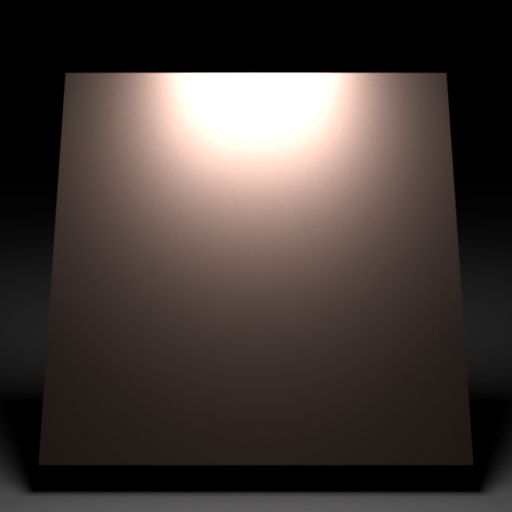
\includegraphics[width=\linewidth]{img/ggx_copper_60.png}
			\caption{Mitsuba2 - reference}
		\end{subfigure}
		&
		\begin{subfigure}
			{0.4\textwidth}\centering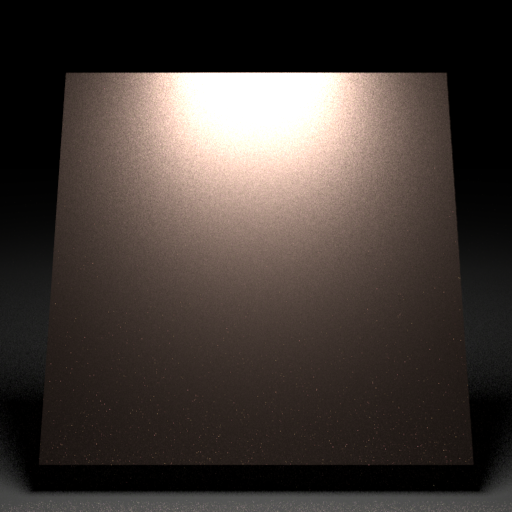
\includegraphics[width=\linewidth]{img/ggx_copper_60_ART.png}
			\caption{ART - our implementation}
		\end{subfigure} \\
		\begin{subfigure}
			{0.4\textwidth}\centering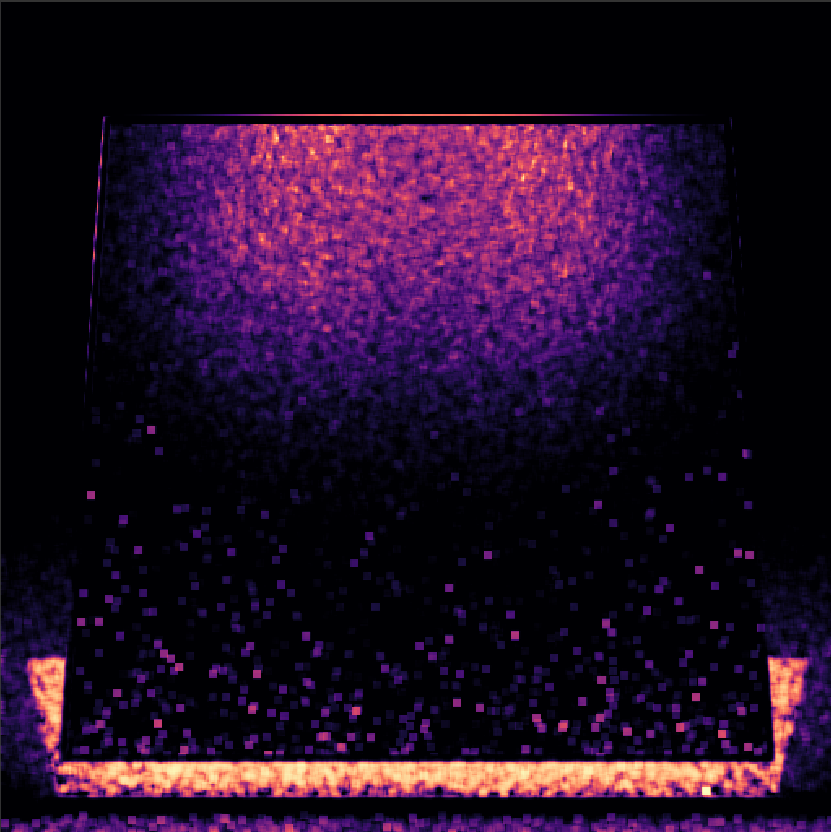
\includegraphics[width=\linewidth]{img/ggx_copper_60_SSIM.png}
			\caption{SSIM}
		\end{subfigure} 
		&
		\begin{subfigure}
			{0.4\textwidth}\centering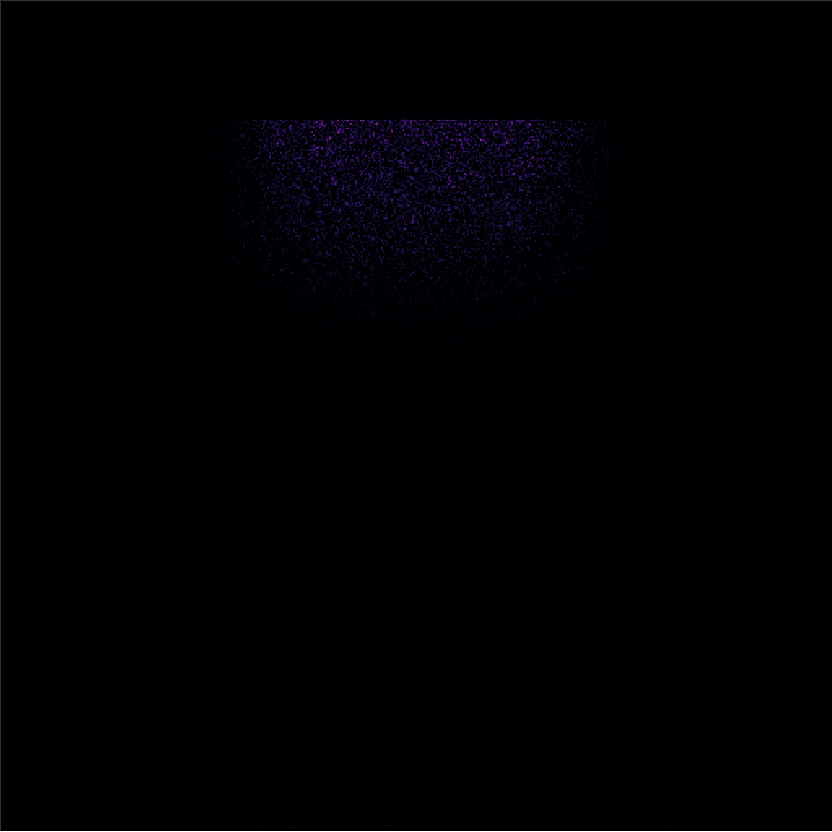
\includegraphics[width=\linewidth]{img/ggx_copper_60_L1.png}
			\caption{L1}
		\end{subfigure}
	\end{tabular}
	\caption{Comparisons between the reference image and the ART implementation of the GGX copper plane (rotated by 60 degrees) scene}
	\label{fig:compare_ggx_copper}
\end{figure}

\renewcommand\thesubfigure{\arabic{subfigure}}
\begin{figure}[h]
	\centering
	\begin{tabular}{cc}
		\begin{subfigure}
			{0.4\textwidth}\centering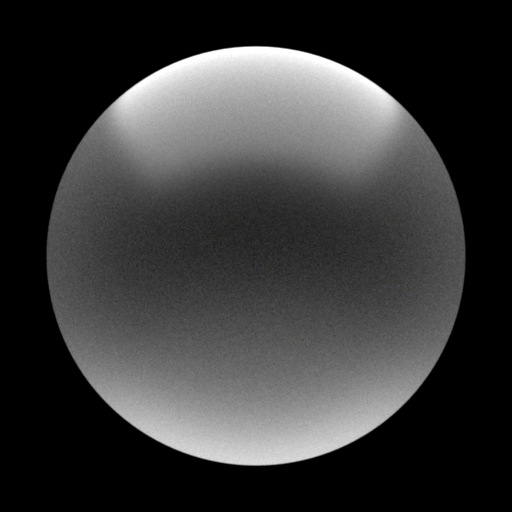
\includegraphics[width=\linewidth]{img/ggx_glass.png}
			\caption{Mitsuba2 - reference}
		\end{subfigure}
		&
		\begin{subfigure}
			{0.4\textwidth}\centering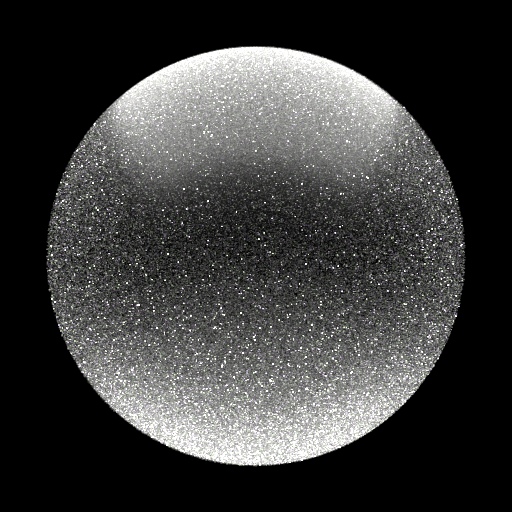
\includegraphics[width=\linewidth]{img/ggx_glass_ART.png}
			\caption{ART - our implementation}
		\end{subfigure} \\
		\begin{subfigure}
			{0.4\textwidth}\centering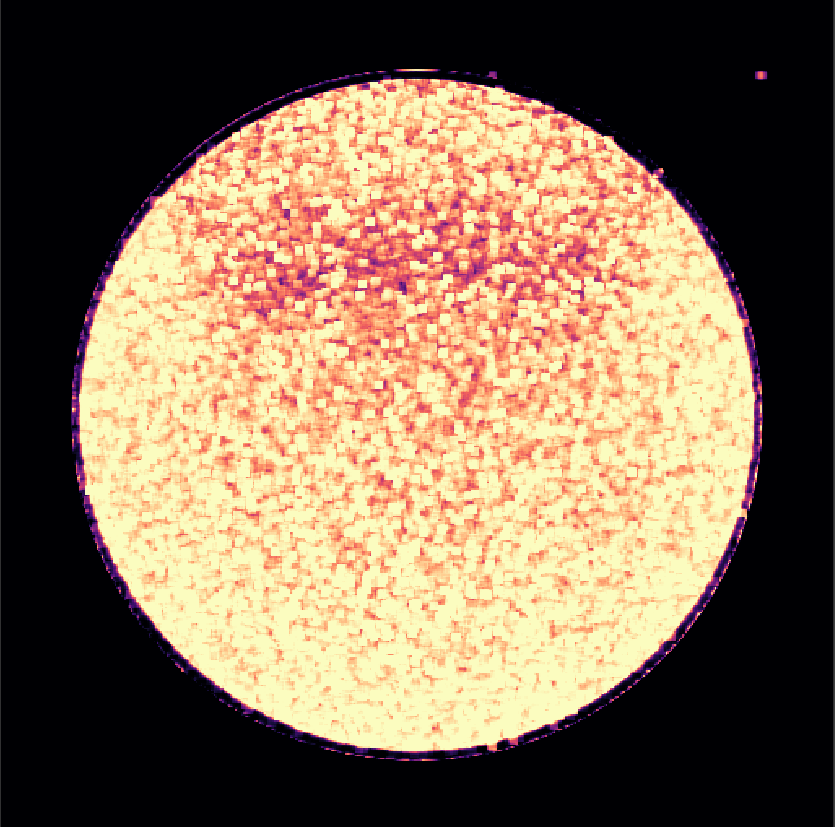
\includegraphics[width=\linewidth]{img/ggx_glass_SSIM.png}
			\caption{SSIM}
		\end{subfigure} 
		&
		\begin{subfigure}
			{0.4\textwidth}\centering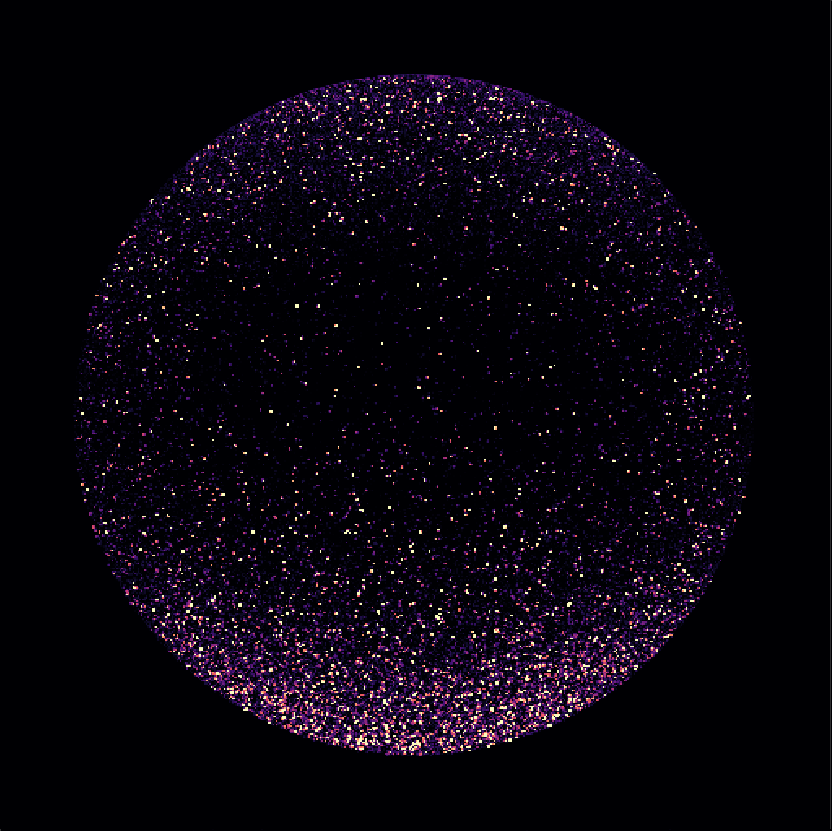
\includegraphics[width=\linewidth]{img/ggx_glass_L1.png}
			\caption{L1}
		\end{subfigure}
	\end{tabular}
	\caption{Comparisons between the reference image and the ART implementation of the GGX glass scene}
	\label{fig:compare_ggx_glass}
\end{figure}

We should note that Mitsuba2 actually implements the improved variant of GGX developed by \citet{heitz2018sampling} which significantly reduces variance. We implemented the original, basic variant~\cite{walter2007microfacet} which logically creates lots of noise for the same amount of samples. Consequently, this diminishes the usability of the SSIM method as the result simply could not converge to the correct state. This is true especially for the glass sphere as there are lot more reflections under various angles than on a simple plane.

However, the L1 function nicely shows that our implementation should be correct. In case of the plane, we see only few dots, signaling that some samples might have brighter colors. In case of the sphere, we can see a larger groups of the dots at the bottom, which is probably caused by the general rough surface model and not the microfacet distribution, as the colors match.

\section{Spectral Accuracy}

The spectral accuracy is significantly harder to quantify and measure as there are lots of mechanisms inside a rendering system that might influence the final colors. Both testing scenes for the spectral accuracy are compared in \autoref{fig:compare_macbeth_d65} and \autoref{fig:compare_macbeth_d50}.

\renewcommand\thesubfigure{\arabic{subfigure}}
\begin{figure}[h]
	\centering
	\begin{tabular}{cc}
		\begin{subfigure}
			{0.4\textwidth}\centering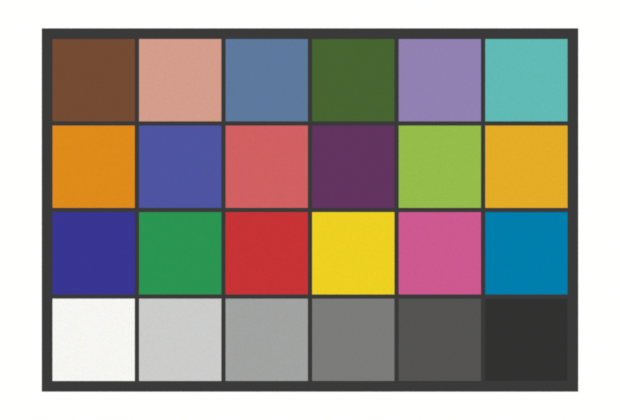
\includegraphics[width=\linewidth]{img/macbeth_chart_D65.png}
			\caption{Mitsuba2 - reference}
		\end{subfigure}
		&
		\begin{subfigure}
			{0.4\textwidth}\centering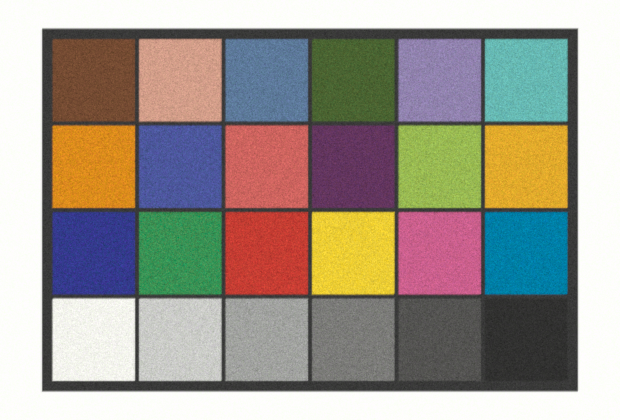
\includegraphics[width=\linewidth]{img/macbeth_chart_D65_ART.png}
			\caption{ART - our implementation}
		\end{subfigure} \\
		\begin{subfigure}
			{0.4\textwidth}\centering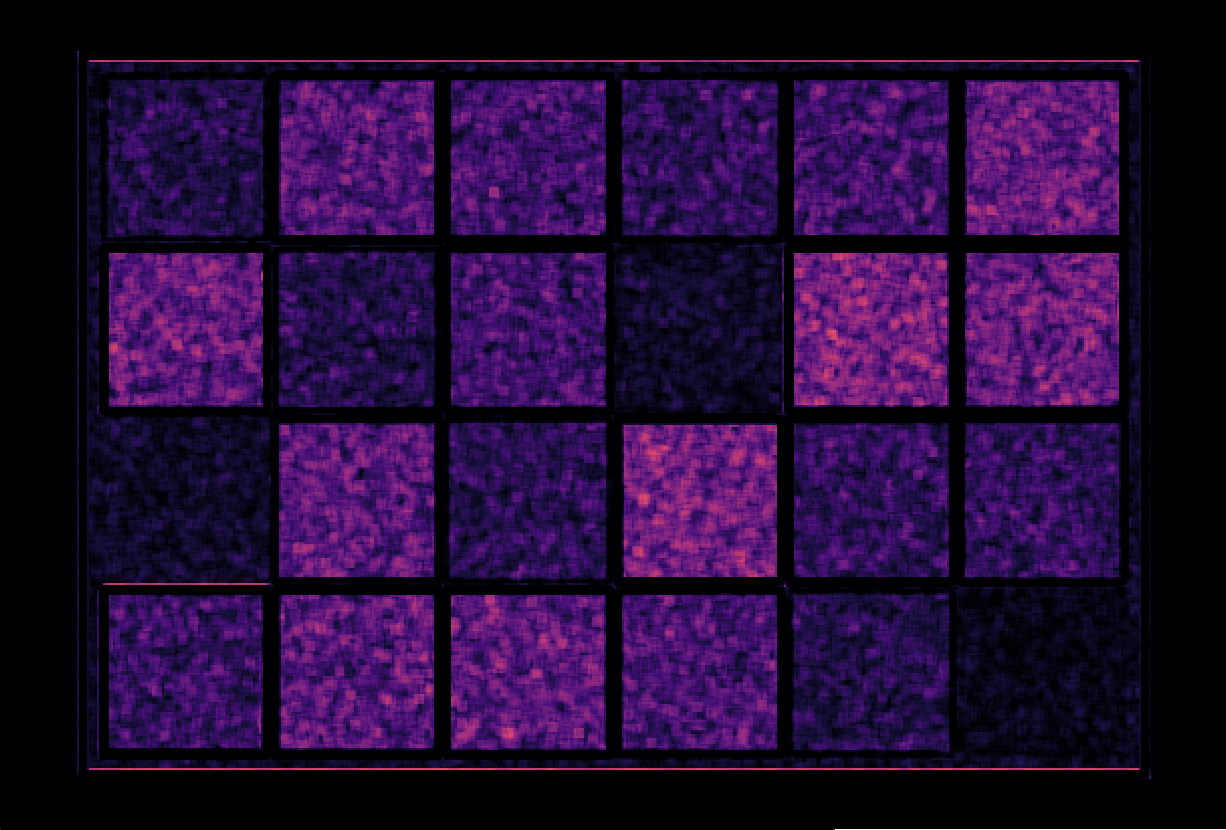
\includegraphics[width=\linewidth]{img/macbeth_chart_D65_SSIM.png}
			\caption{SSIM}
		\end{subfigure} 
		&
		\begin{subfigure}
			{0.4\textwidth}\centering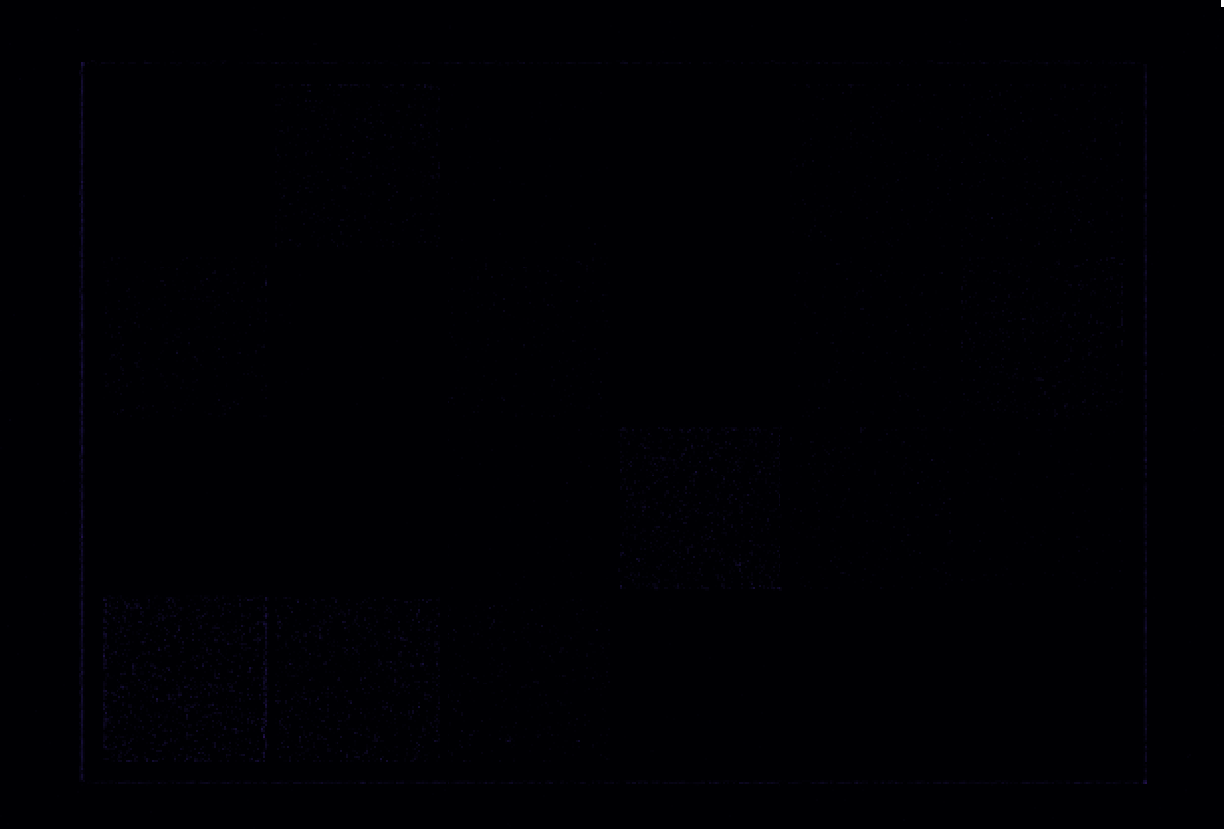
\includegraphics[width=\linewidth]{img/macbeth_chart_D65_L1.png}
			\caption{L1}
		\end{subfigure}
	\end{tabular}
	\caption{Comparisons between the reference image and the ART implementation of the Macbeth chart D65 scene}
	\label{fig:compare_macbeth_d65}
\end{figure}

\renewcommand\thesubfigure{\arabic{subfigure}}
\begin{figure}[h]
	\centering
	\begin{tabular}{cc}
		\begin{subfigure}
			{0.4\textwidth}\centering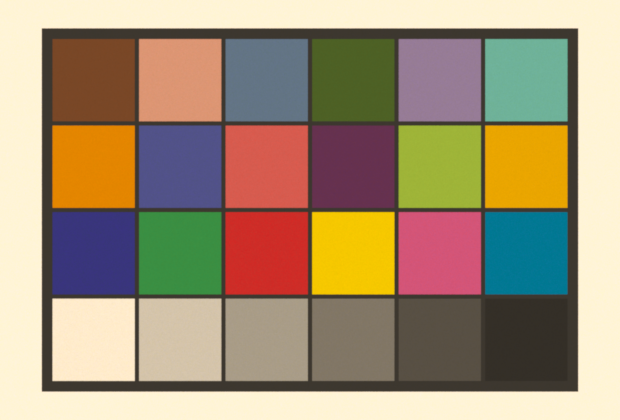
\includegraphics[width=\linewidth]{img/macbeth_chart_D50.png}
			\caption{Mitsuba2 - reference}
		\end{subfigure}
		&
		\begin{subfigure}
			{0.4\textwidth}\centering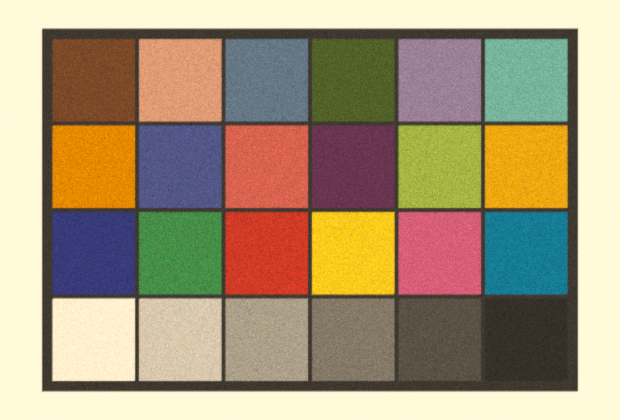
\includegraphics[width=\linewidth]{img/macbeth_chart_D50_ART.png}
			\caption{ART - our implementation}
		\end{subfigure} \\
		\begin{subfigure}
			{0.4\textwidth}\centering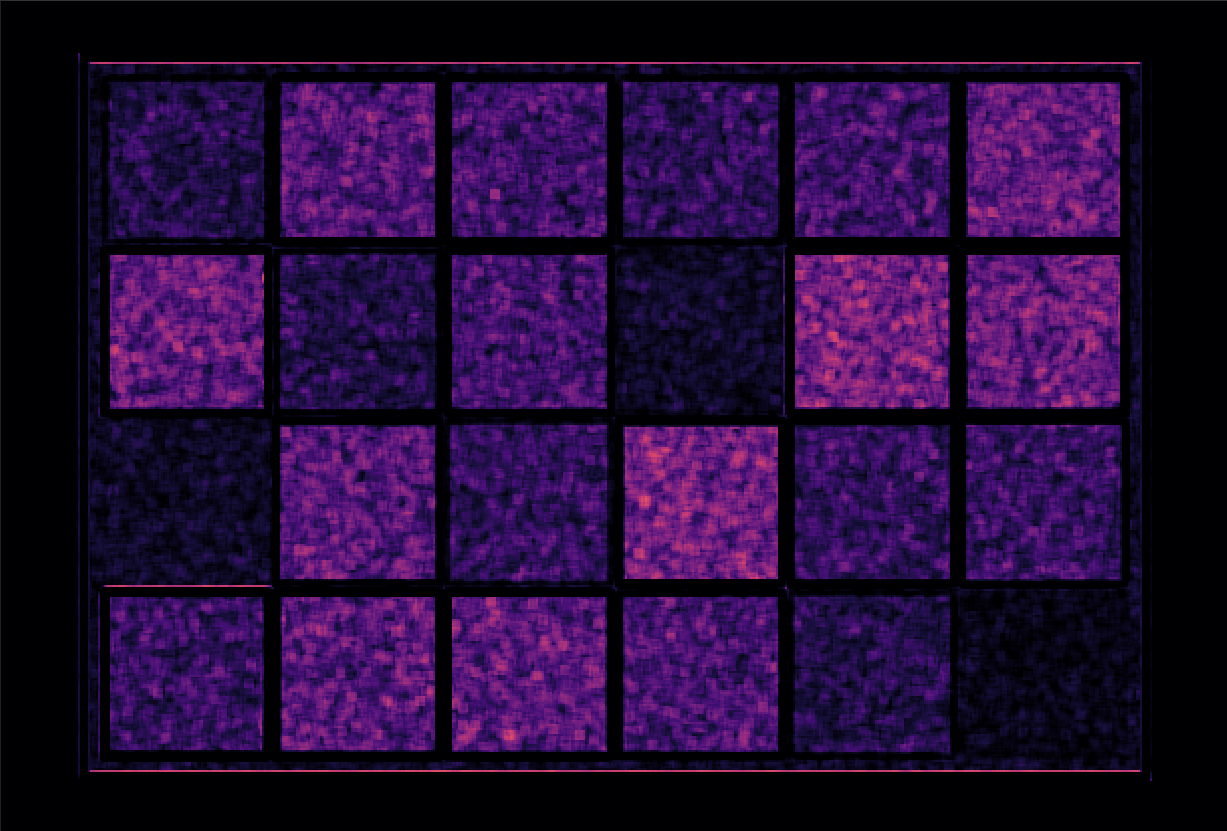
\includegraphics[width=\linewidth]{img/macbeth_chart_D50_SSIM.png}
			\caption{SSIM}
		\end{subfigure} 
		&
		\begin{subfigure}
			{0.4\textwidth}\centering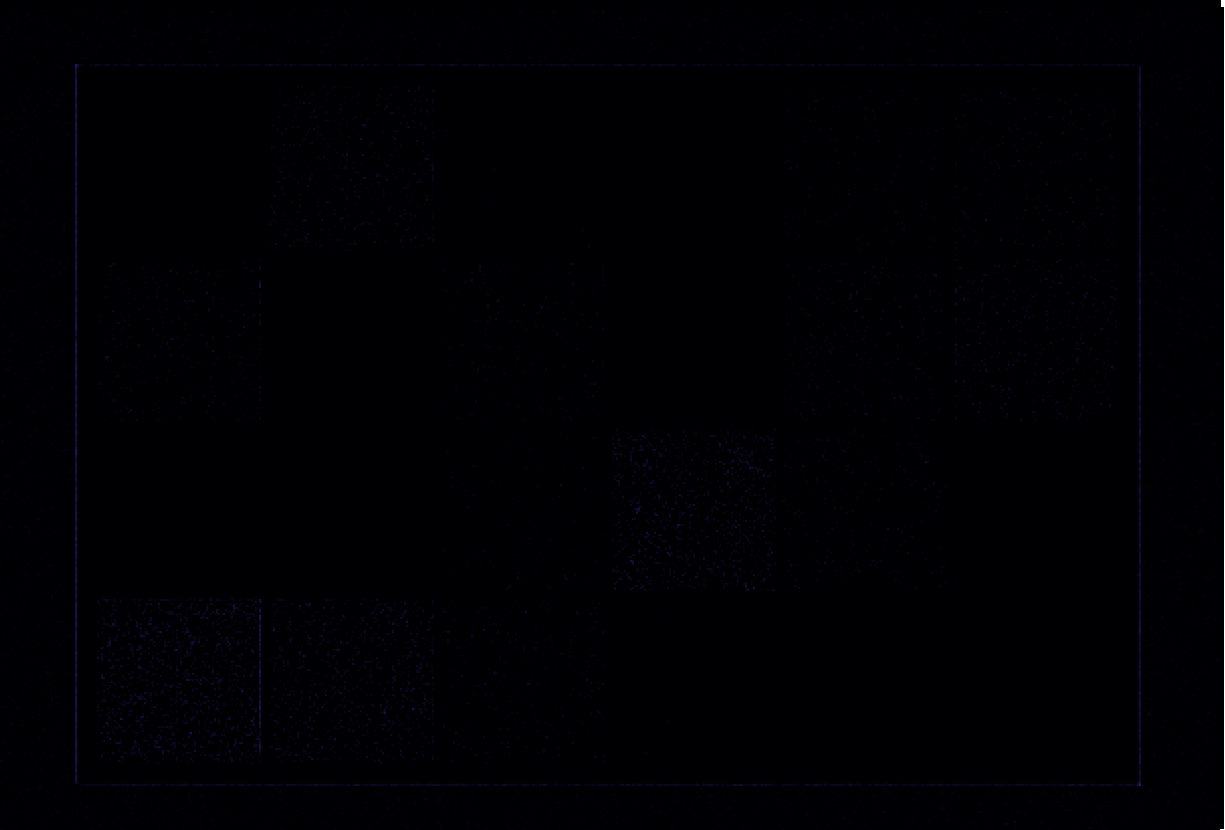
\includegraphics[width=\linewidth]{img/macbeth_chart_D50_L1.png}
			\caption{L1}
		\end{subfigure}
	\end{tabular}
	\caption{Comparisons between the reference image and the ART implementation of the Macbeth chart D50 scene}
	\label{fig:compare_macbeth_d50}
\end{figure}

On the first sight, the two images are extremely similar --- the spectral definitions for the Macbeth colors and the illuminants are the very same for both renderers. This is also proved by the L1 comparisons which shows almost no difference. But as we look on the SSIM, we see slight variations in different color patches. The Macbeth blue and black are accurate but for some reason the others, especially the yellow and yellow-green are slightly more saturated in the reference images. This might indicate a potential flow in the stochastic approach of spectral sampling in Mitsuba2 but as the differences are barely there, we do not consider the results to be incorrect. Note that the two SSIM images are almost identical which shows that the relative comparison under the same lighting conditions matches.  

\section{Polarization}

Unfortunately for us, the comparison between the Stokes vector outputs heavily depend on the viewer and the representation of the specific renderer. To make the matters as simple as possible, the scene is monochrome and tracks a single-wavelength light only. We show the comparisons of the second Stokes vector element --- the horizontal/vertical polarization --- in \autoref{fig:compare_polar_s1} and the comparisons of the scene with the visible polarized reflection in \autoref{fig:compare_polar_angle}.

\renewcommand\thesubfigure{\arabic{subfigure}}
\begin{figure}[h]
	\centering
	\begin{tabular}{cc}
		\begin{subfigure}
			{0.4\textwidth}\centering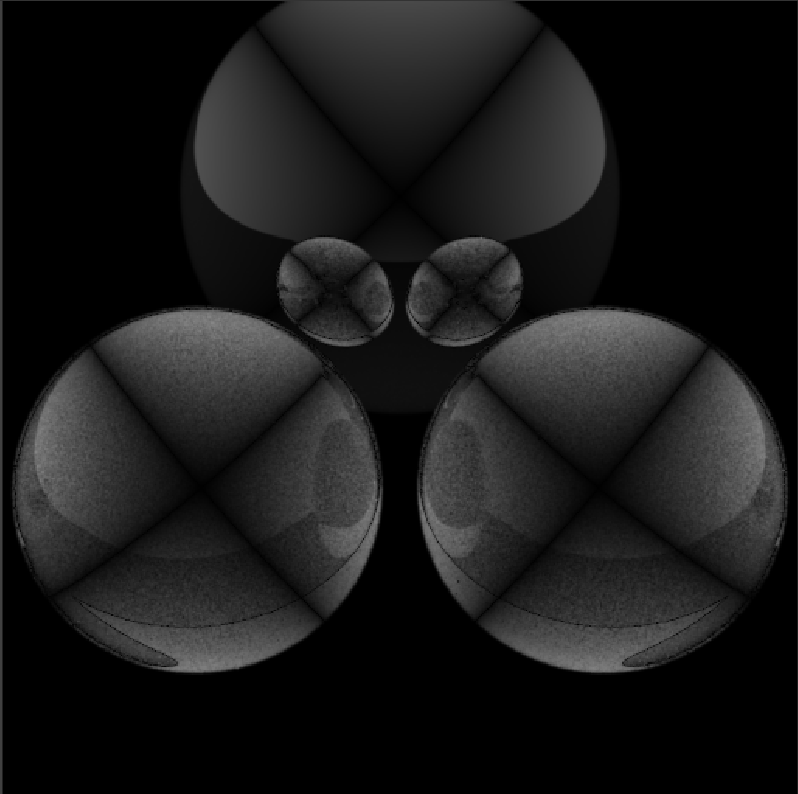
\includegraphics[width=\linewidth]{img/polarizing_spheres.s1.png}
			\caption{Mitsuba2 - reference}
		\end{subfigure}
		&
		\begin{subfigure}
			{0.4\textwidth}\centering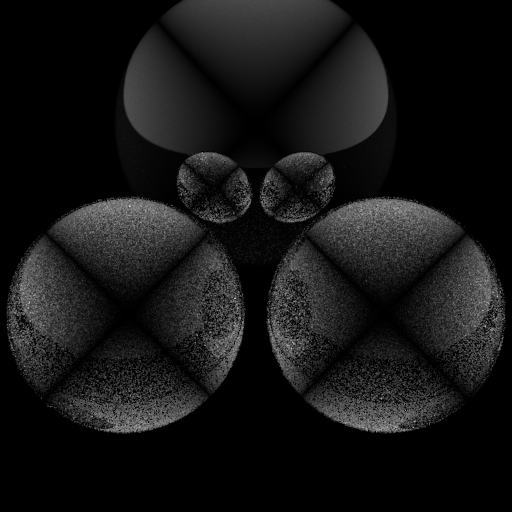
\includegraphics[width=\linewidth]{img/polarizing_spheres.s1_ART.png}
			\caption{ART - our implementation}
		\end{subfigure} \\
		\begin{subfigure}
			{0.4\textwidth}\centering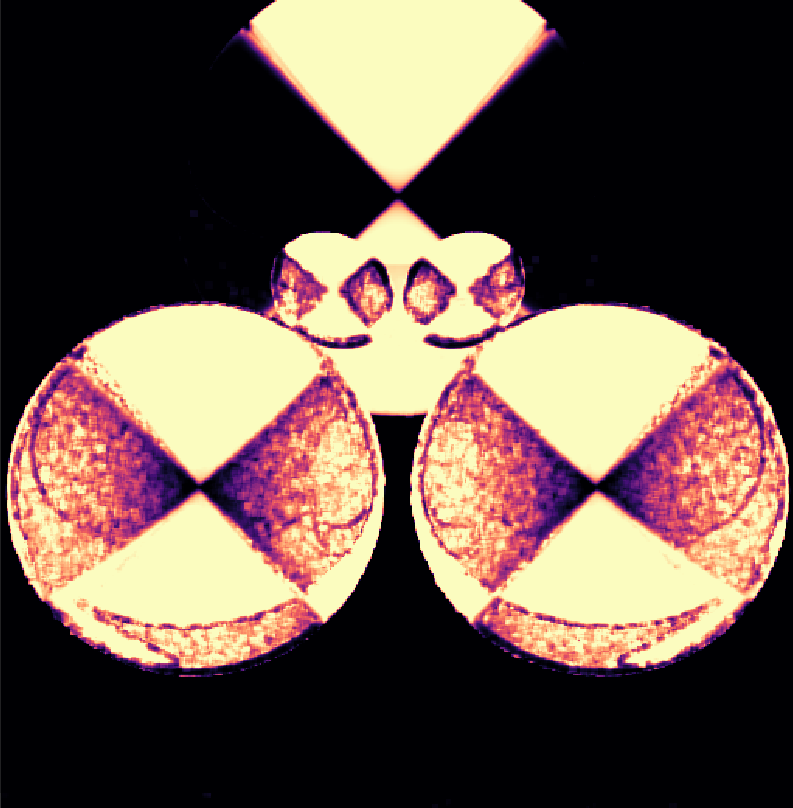
\includegraphics[width=\linewidth]{img/polarizing_spheres.s1_SSIM.png}
			\caption{SSIM}
		\end{subfigure} 
		&
		\begin{subfigure}
			{0.4\textwidth}\centering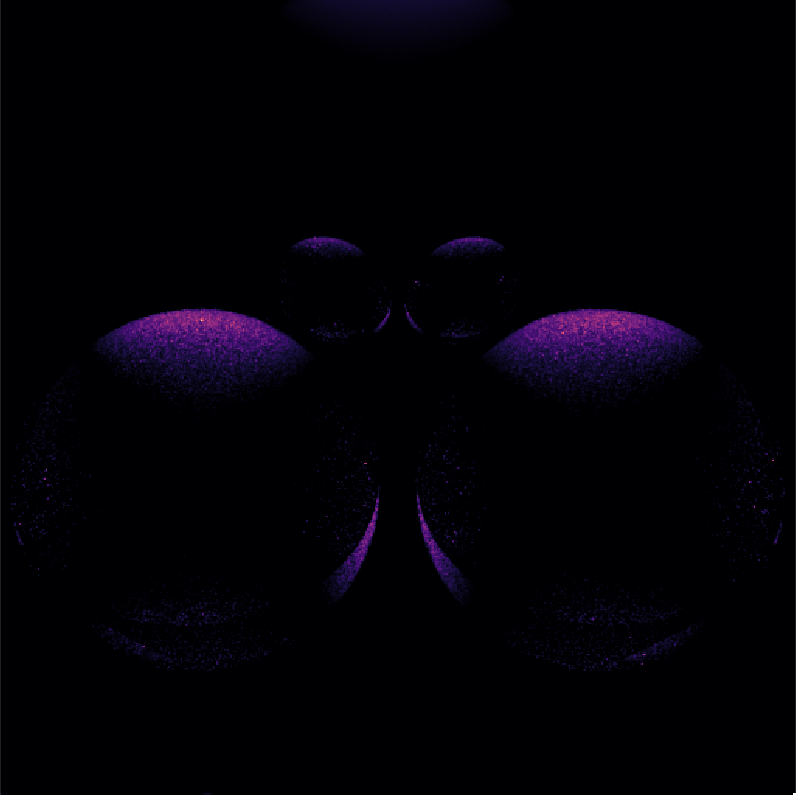
\includegraphics[width=\linewidth]{img/polarizing_spheres.s1_L1.png}
			\caption{L1}
		\end{subfigure}
	\end{tabular}
	\caption{Comparisons between the reference image and the ART implementation of the second Stokes vector element of the polarizing spheres scene}
	\label{fig:compare_polar_s1}
\end{figure}

\renewcommand\thesubfigure{\arabic{subfigure}}
\begin{figure}[h]
	\centering
	\begin{tabular}{cc}
		\begin{subfigure}
			{0.4\textwidth}\centering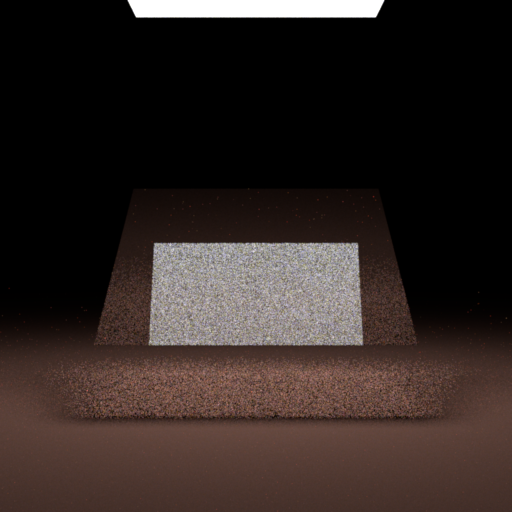
\includegraphics[width=\linewidth]{img/polarizing_plane_90.png}
			\caption{Mitsuba2 - reference}
		\end{subfigure}
		&
		\begin{subfigure}
			{0.4\textwidth}\centering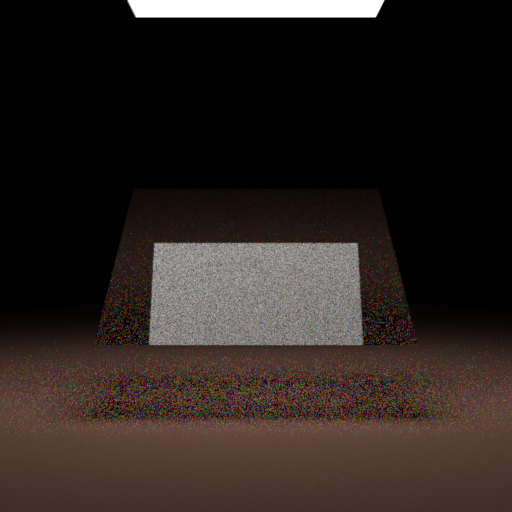
\includegraphics[width=\linewidth]{img/polarizing_plane_90_ART.png}
			\caption{ART - our implementation}
		\end{subfigure} \\
		\begin{subfigure}
			{0.4\textwidth}\centering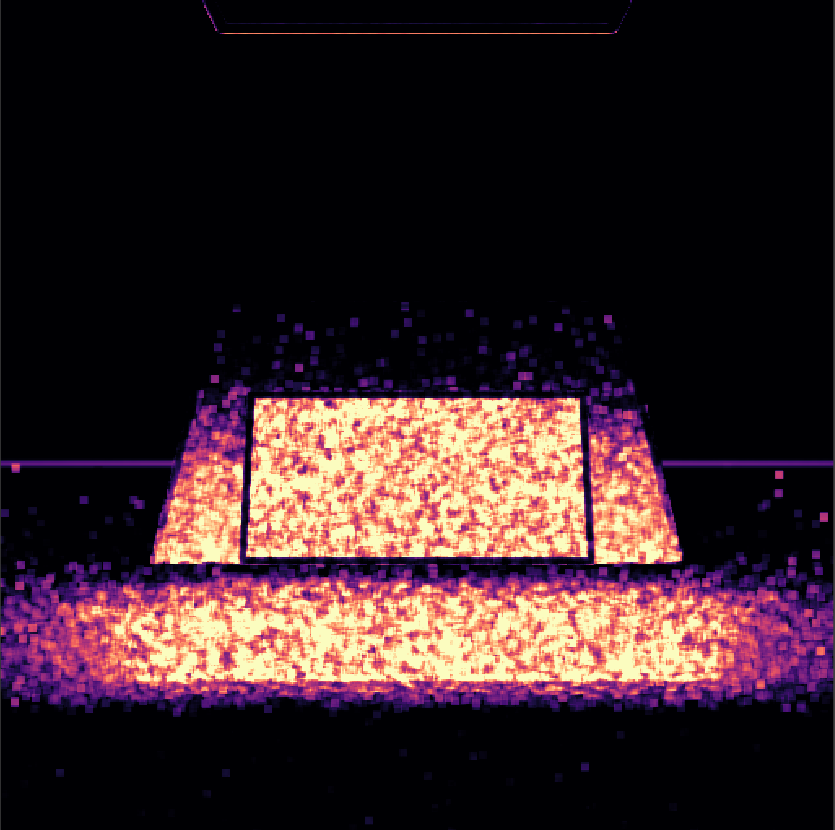
\includegraphics[width=\linewidth]{img/polarizing_plane_90_SSIM.png}
			\caption{SSIM}
		\end{subfigure} 
		&
		\begin{subfigure}
			{0.4\textwidth}\centering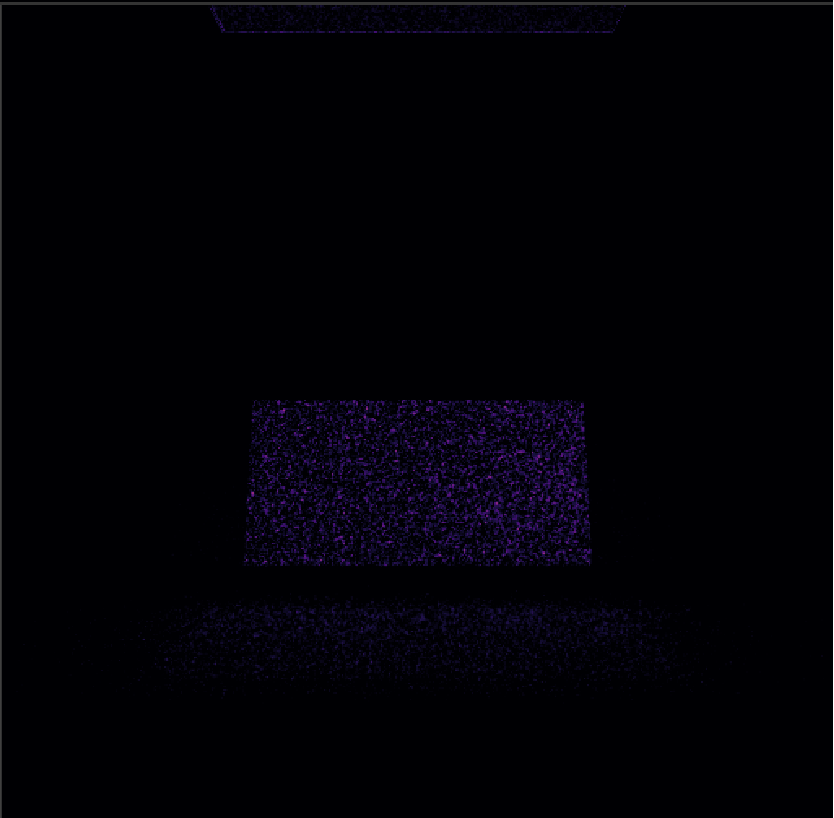
\includegraphics[width=\linewidth]{img/polarizing_plane_90_L1.png}
			\caption{L1}
		\end{subfigure}
	\end{tabular}
	\caption{Comparisons between the reference image and the ART implementation of the polarizing plane (filter rotated by 90 degrees) scene}
	\label{fig:compare_polar_angle}
\end{figure}

The polarizing plane scene might seem to be more attenuated in case of ART, especially under the plane. However, this does not concern us as the purpose of the scene is to expose the behavior of the unpolarized light upon the interaction with a surface under a Brewster's angle rather than the material properties and the transmissions through them. Neither of the difference images show an obvious inconsistency between the images but both are suggesting that the reflection of the light on the plane is at least partially off.

With the simplifications of the polarizing sphere scene we've mentioned above, we can see that the results are almost identical. But, there is  a visible difference in the vertical polarization on the spheres (properly exposed by SSIM) and we could conclude that there are some errors as the light is not actually unpolarized in case of Mitsuba2. However, bear in mind that the images we compare are not a direct results of the rendering process but rather a byproduct of a specific structure inside it.